\section{Results}
\label{sect:results}

\subsection{Integrity and the Single-Peak Domain}

All 23\,000 native-schedule fits and all 11\,040 matched-$N$ fits converged successfully and satisfy the final scientific-validity checks. No multi-peak epoch occurs anywhere in either final grid. The results reported in this section therefore characterize a single-peak response regime; they are not produced by assigning one coordinate to a visibly split two-mode profile.

\subsection{Light-Fraction and Separation Dependence}

Figure~\ref{fig:surface} shows the native full-sky median discrepancy over the $(\betag,\asig)$ grid. The response is non-monotonic in light fraction. For every one of the 46 sky positions and each of the five tested separations, the largest median $\dchi$ occurs at $\betag=0.25$, i.e. in 230/230 sky/separation combinations. The reduced matched-$N$ grid independently gives the same result for all 184/184 combinations for which $\betag=0.05,0.25,0.45$ were compared.

The fall-off toward $\betag\rightarrow0$ is expected because a dark secondary contributes no second light-profile component. The decrease toward equal light is also expected from symmetry: for an exact equal-light profile in the single-peak domain, the central maximum coincides with the flux-weighted photocentre. The most visible disagreement therefore occurs at intermediate light fraction.

\begin{figure}
\centering
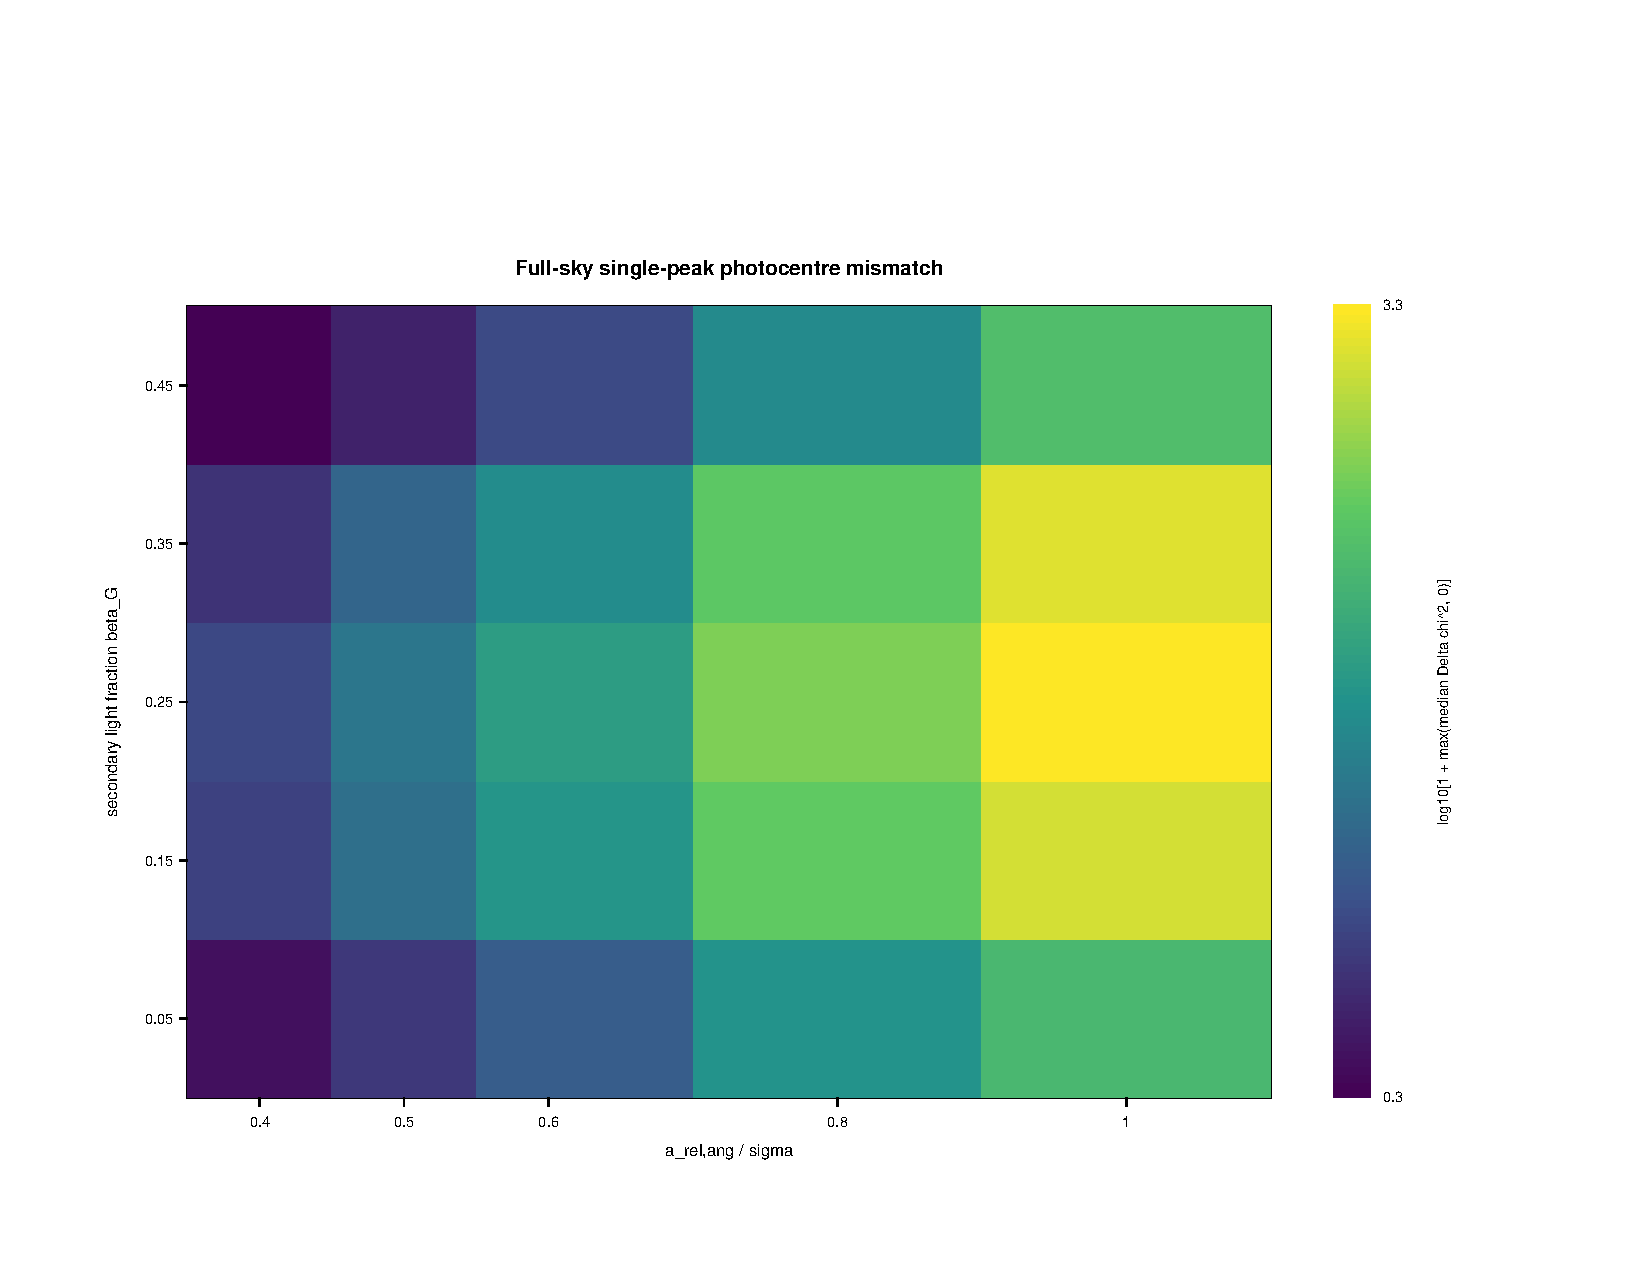
\includegraphics[width=0.92\textwidth]{figures/full_sky_dr4_beta_separation_surface}
\caption{Full-sky native-schedule photocentre--RAA mismatch in the single-peak domain. Each cell is the median paired $\dchi$ over all sky positions and noise seeds, displayed logarithmically. The surrogate width $\sigma$ is a research scale and the horizontal coordinate is not a Gaia resolution threshold.}
\label{fig:surface}
\end{figure}

\subsection{Full-Sky Variation}

At $\betag=0.25$ and $\asig=1$, the sky distribution of median $\dchi$ has minimum 834.14, median 2195.39, and maximum 8766.64. The native $Q_{16}(\dchi)>0$ boundary first occurs at the smallest sampled ratio, $\asig=0.40$, for 41/46 positions, while the remaining five first cross at 0.50. Requiring all ten realizations at a sky position to have $\dchi>0$ moves the first crossing to 0.40 for 18 positions, 0.50 for 23, and 0.60 for five. These are descriptive sampled boundaries rather than formal detection thresholds.

At the same $(\betag,\asig)$ point the Spearman rank correlation between median $\dchi$ and native transit count is
\begin{equation}
\rho_{\rm S}=0.7709.
\end{equation}
The corresponding correlations with maximum directional scan-angle gap and normalized directional entropy are $-0.640$ and $+0.358$, respectively. The native sky dependence therefore combines observation count and scan geometry.

\begin{figure}
\centering
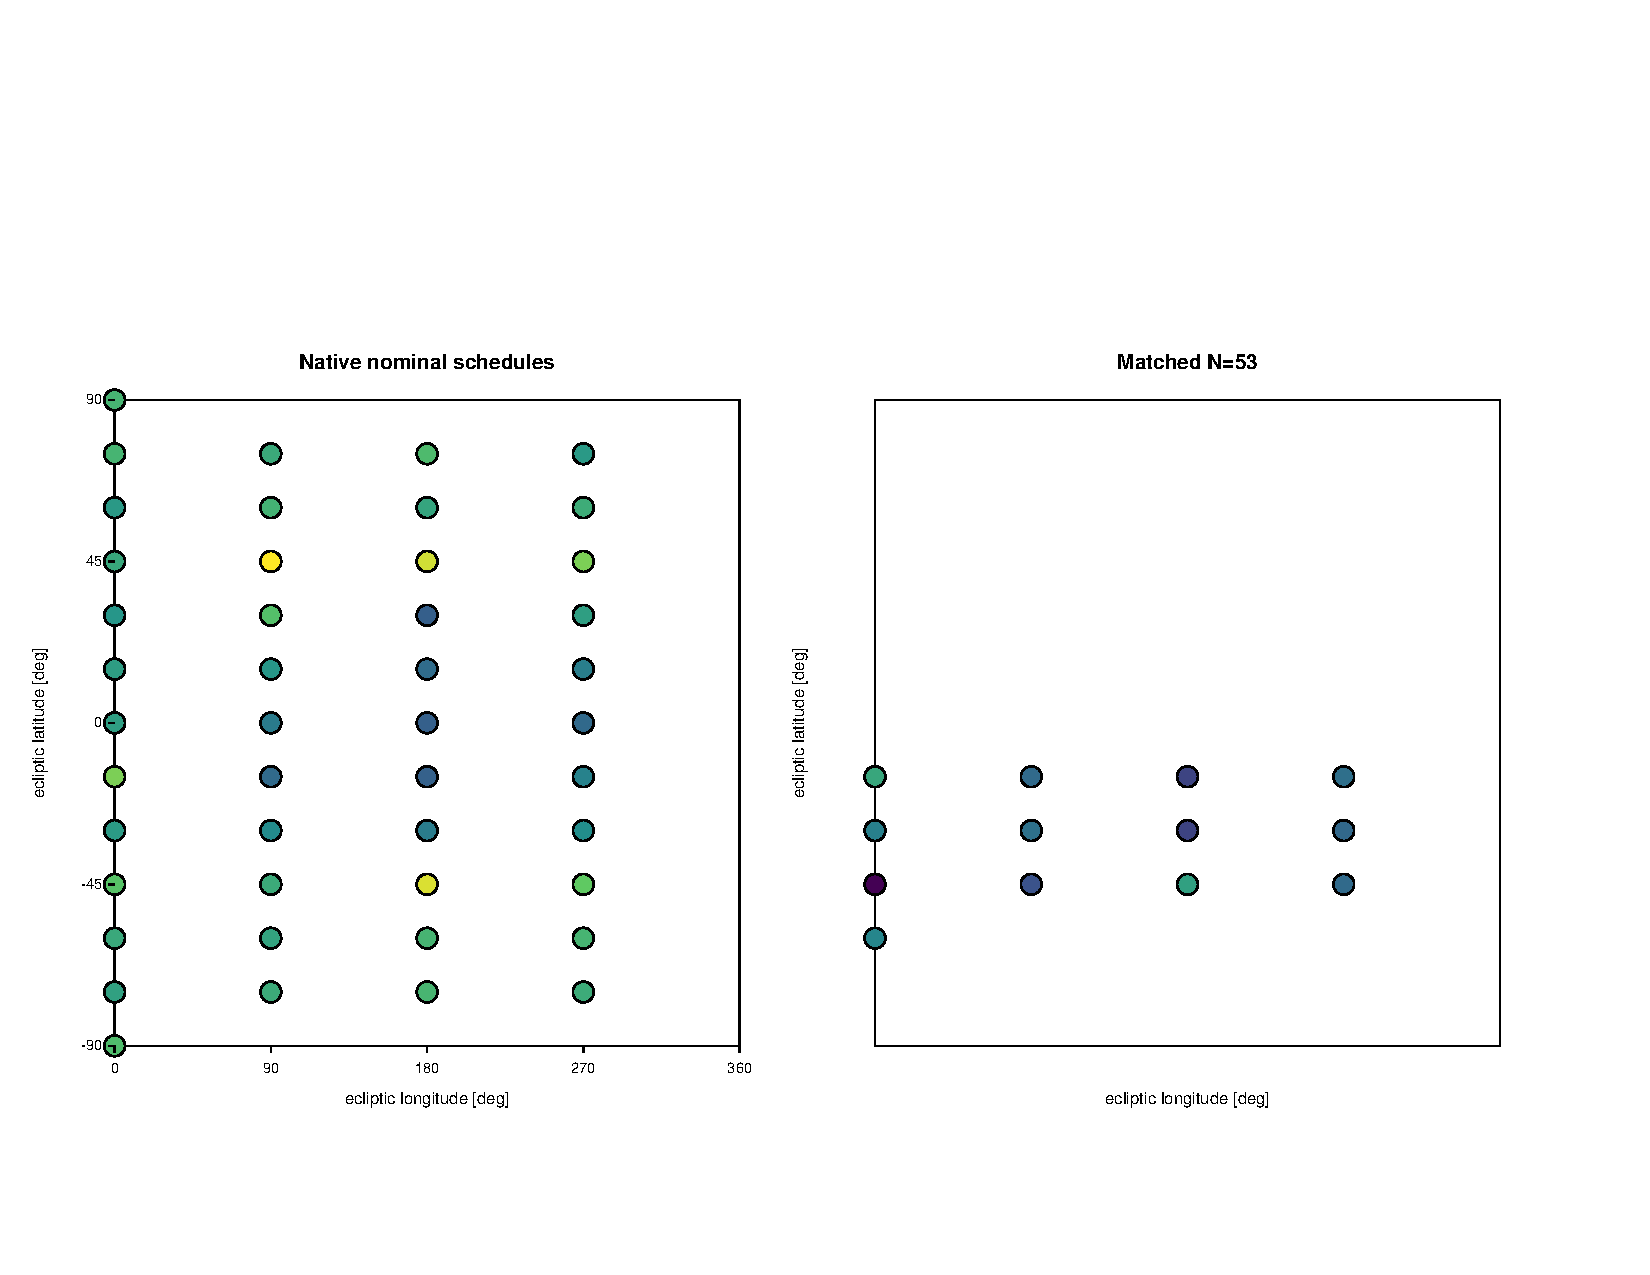
\includegraphics[width=0.98\textwidth]{figures/full_sky_dr4_native_matched_sky}
\caption{Sampled ecliptic-sky maps of the median paired $\dchi$ for $\betag=0.25$ and $\asig=1$, using the same logarithmic colour normalization. The left panel uses the native nominal schedules with 53--310 transits; the right panel uses the matched schedules with exactly 53 transits.}
\label{fig:skymaps}
\end{figure}

\subsection{Matched-Transit-Count Control}

Fixing all positions to $N=53$ reduces the sky-median $\dchi$ from 2195.39 to 1180.94, a ratio of 0.5379. The matched sky range is 300.04--2230.26, substantially narrower than the native 834.14--8766.64 range. Most importantly, the correlation with the \emph{native} transit count becomes
\begin{equation}
\rho_{\rm S}(\dchi_{53},N_{\rm native})=-0.0032,
\end{equation}
consistent with no monotonic relation. This shows directly that the strong native correlation was driven by the number of retained measurements rather than merely by another sky property correlated with $N$.

Figure~\ref{fig:nativecontrol} compares native and matched values at each sky position. High-$N$ native schedules generally move furthest below the one-to-one line when reduced to 53 measurements.

\begin{figure}
\centering
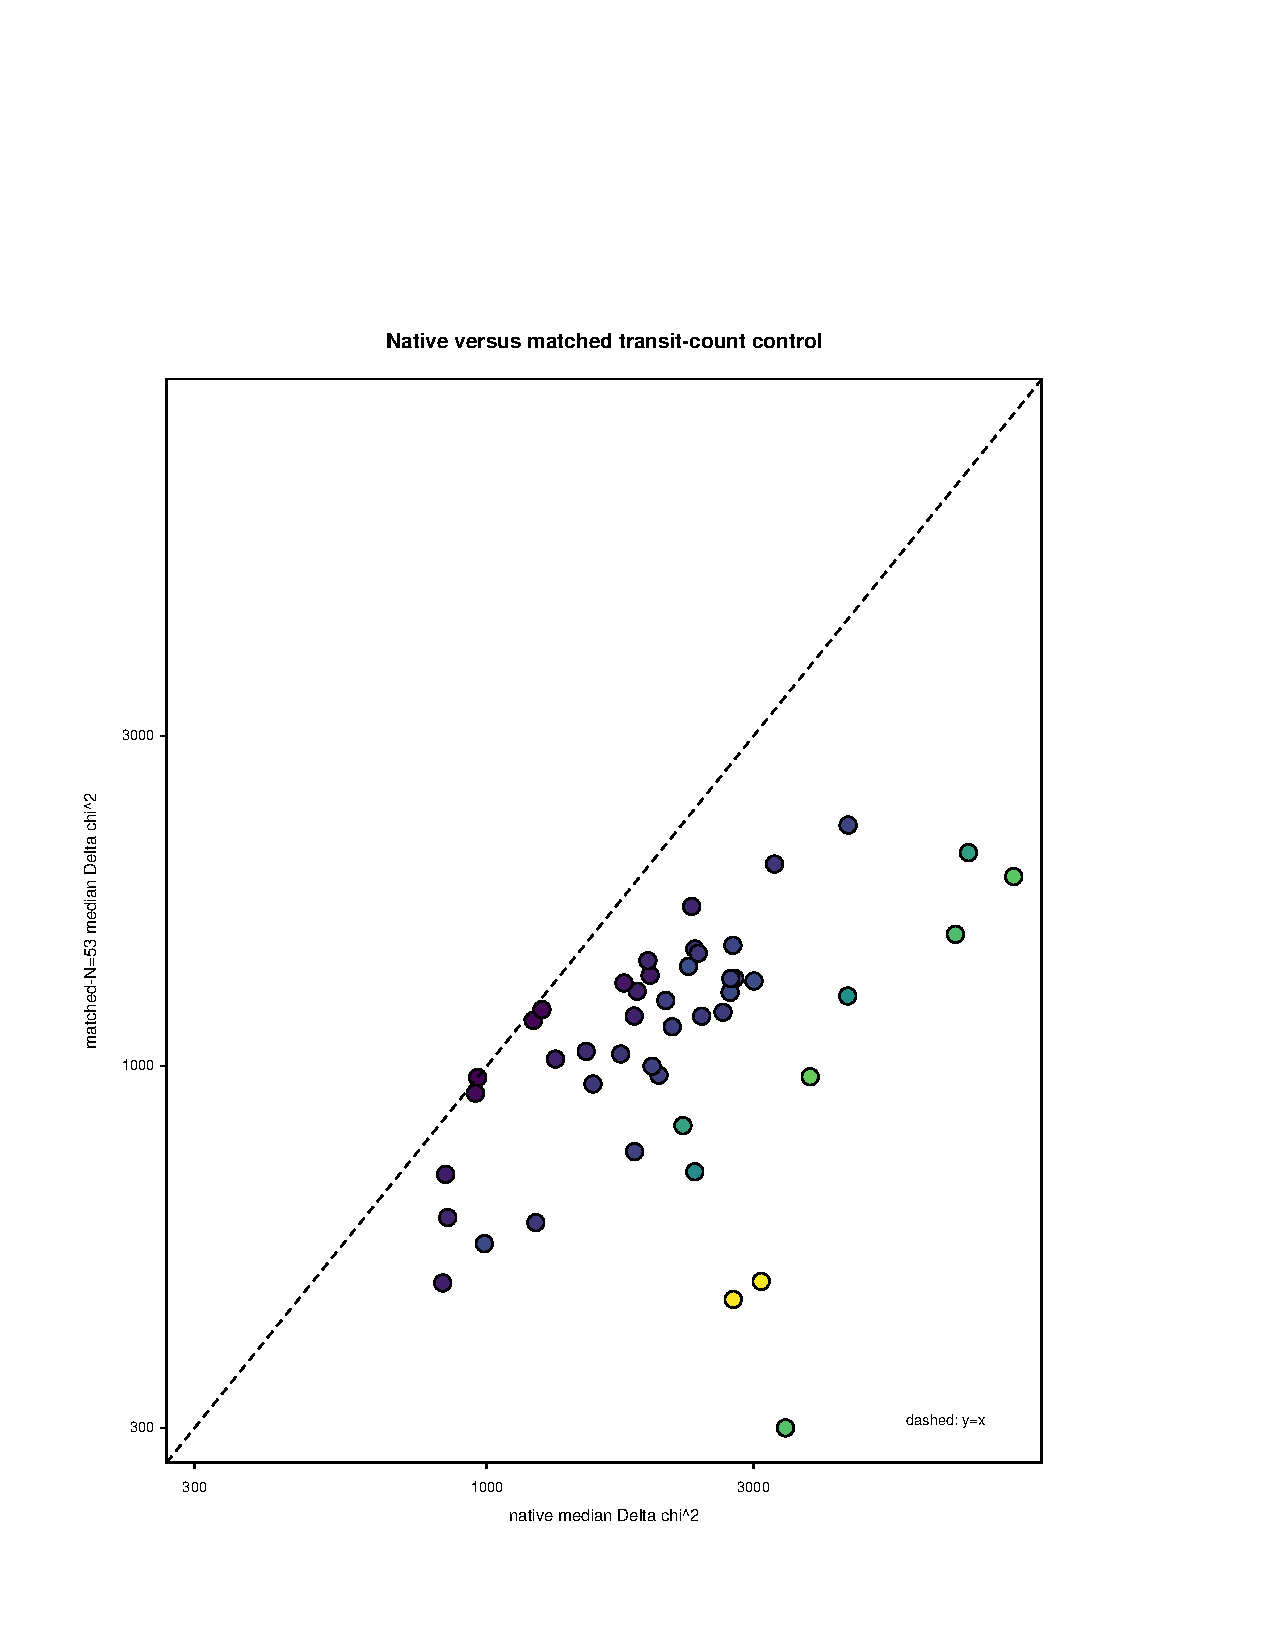
\includegraphics[width=0.80\textwidth]{figures/full_sky_dr4_native_vs_matched_n53}
\caption{Native versus matched-$N=53$ median $\dchi$ across the 46 sky positions for $\betag=0.25$ and $\asig=1$. Colour denotes the native nominal transit count. The dashed line is equality.}
\label{fig:nativecontrol}
\end{figure}

The ratio of model discrepancies closely follows the fraction of transits retained:
\begin{equation}
\rho_{\rm S}\left(
\frac{\dchi_{53}}{\dchi_{\rm native}},
\frac{53}{N_{\rm native}}
\right)=0.9233.
\end{equation}
Furthermore,
\begin{equation}
{\rm median}\left[
\frac{\dchi_{53}/\dchi_{\rm native}}{53/N_{\rm native}}
\right]=1.0138.
\label{eq:scaling}
\end{equation}
The median native discrepancy per transit is 21.44, compared with 22.28 in the matched control. Within this particular synthetic strong-response case, Equation~(\ref{eq:scaling}) is therefore consistent with an approximately linear accumulation of model-discrimination information with the number of Gaia-like observations.

\begin{figure}
\centering
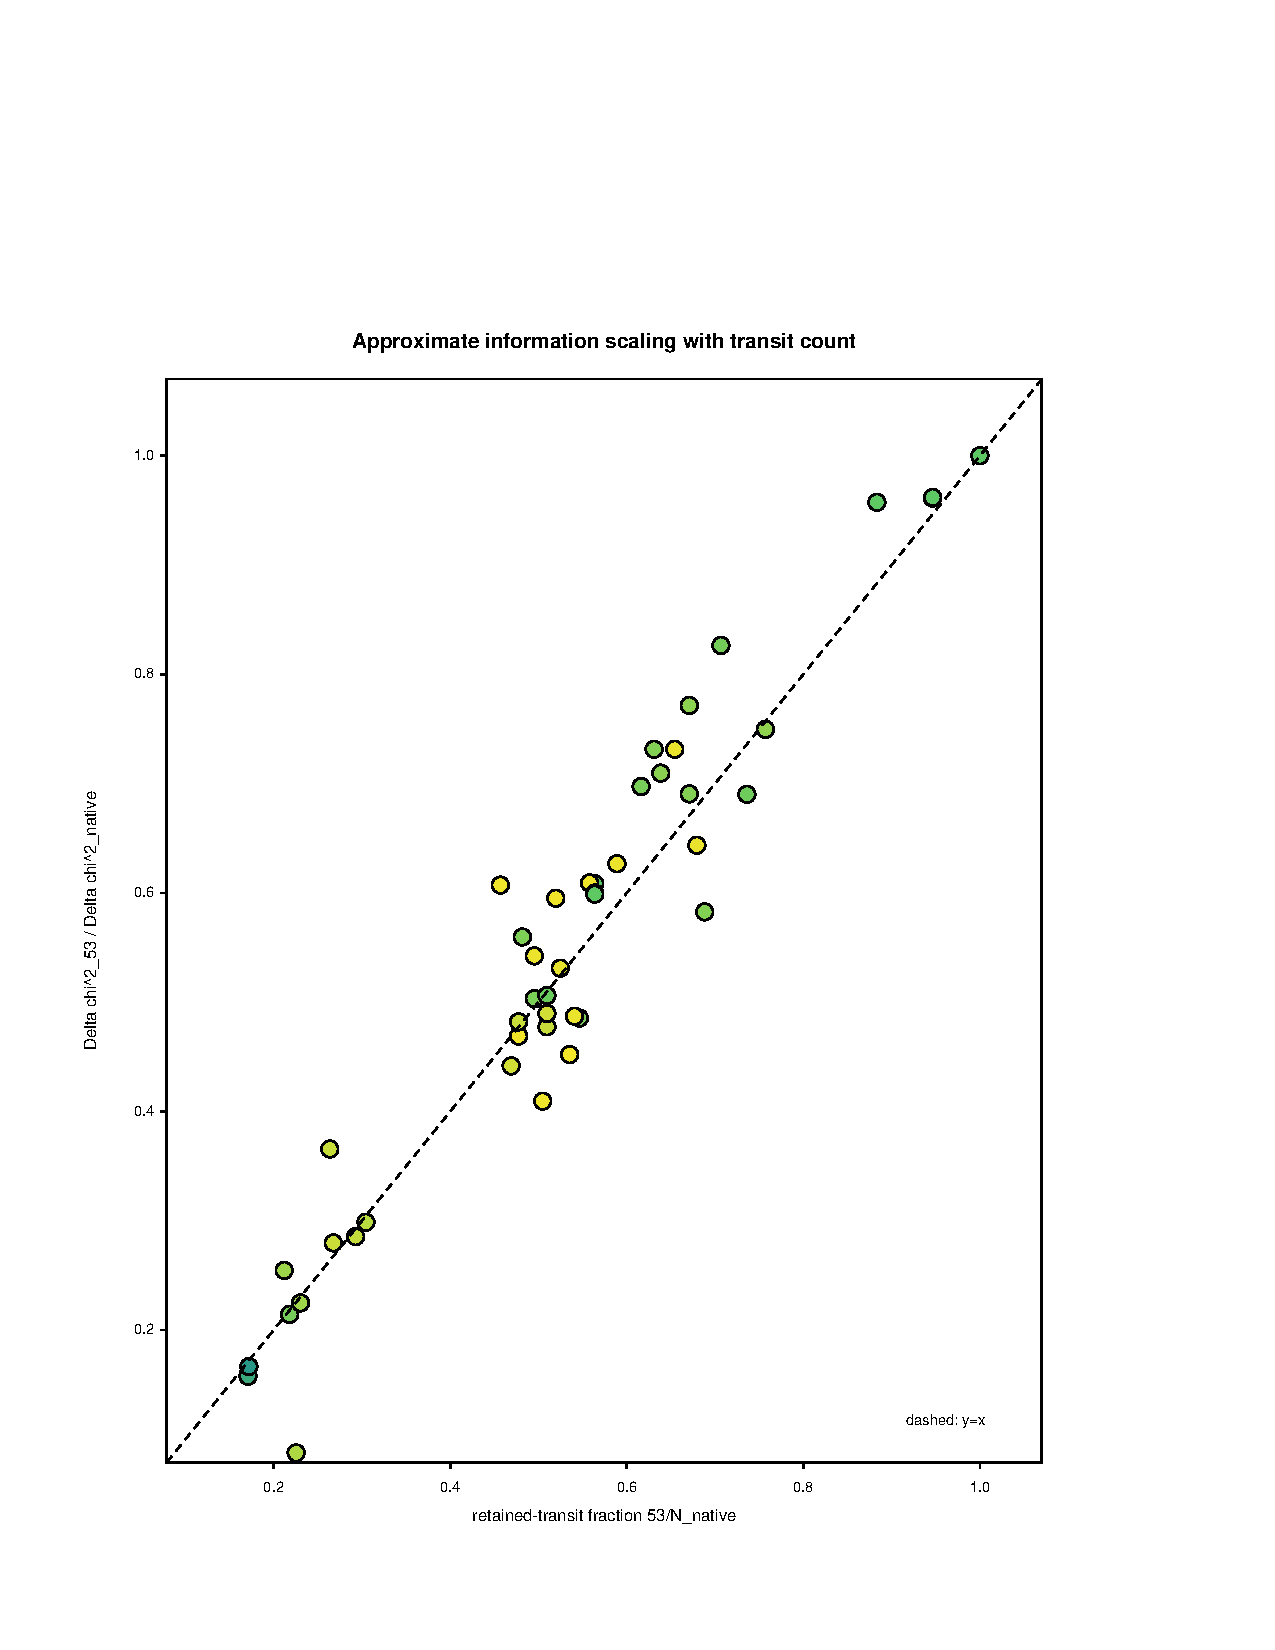
\includegraphics[width=0.80\textwidth]{figures/full_sky_dr4_matched_n53_scaling}
\caption{Ratio of matched to native model discrepancy versus the retained-transit fraction. Each point is one sky position at $\betag=0.25$ and $\asig=1$. The dashed line is the simple proportional scaling $\dchi_{53}/\dchi_{\rm native}=53/N_{\rm native}$; colour denotes the normalized scan-angle entropy of the 53 retained measurements.}
\label{fig:scaling}
\end{figure}

Equalizing the count does not erase all sky dependence. For the same control point, $\rho_{\rm S}(\dchi_{53},H_{\rm angle})=+0.340$ and $\rho_{\rm S}(\dchi_{53},\Delta\psi_{\max})=-0.275$, where $H_{\rm angle}$ is normalized directional entropy and $\Delta\psi_{\max}$ is the maximum directional angular gap. Thus scan geometry leaves a measurable residual contribution after the dominant count effect is removed.

The transition boundary shifts accordingly. At $\betag=0.25$, 31/46 matched positions have $Q_{16}(\dchi)>0$ by $\asig=0.40$ and 15/46 first cross at 0.50. For the stricter all-seeds-positive condition the matched first crossings are 0.40 for eight positions, 0.50 for 24, 0.60 for 13, and 1.00 for one position. Additional observations therefore move the descriptive transition inward for a substantial part of the sky.

\subsection{Bias in Physical Parameters}

The photocentre model can partially absorb a wrong measurement response by changing fitted physical parameters. Pooling all sky positions and seeds at $\asig=1$, the median fractional photocentre bias in $\betag$ is $-22.6\%$, $-18.0\%$, $-12.6\%$, $-7.17\%$, and $-2.12\%$ for $\betag=0.05,0.15,0.25,0.35,0.45$, respectively. For the central $\betag=0.25$ case, the median photocentre mass biases pooled over the full sky are approximately $-0.61\%$ for $M_1$ and $-0.66\%$ for $M_2$, while the median parallax bias is $+0.51\%$. Across individual sky positions, the median $\betag$ bias ranges from $-19.3\%$ to $-8.0\%$, whereas median mass biases remain within about $-1.6\%$ to $+0.9\%$.

This separation is informative: the parameter with the largest fractional bias need not coincide with the light fraction that maximizes $\dchi$. Model-discrimination strength and parameter-bias amplitude are distinct diagnostics.

\begin{table}
\begin{center}
\caption{Key Full-Sky and Matched-$N$ Results at $\betag=0.25$, $\asig=1$}
\label{tab:results}
\begin{tabular}{lcc}
\hline\noalign{\smallskip}
Quantity & Native schedules & Matched $N=53$\\
\hline\noalign{\smallskip}
Fit records in experiment & 23\,000 & 11\,040\\
Sky positions & 46 & 46\\
Transit count & 53--310 & 53\\
Sky min median $\dchi$ & 834.14 & 300.04\\
Sky median median $\dchi$ & 2195.39 & 1180.94\\
Sky max median $\dchi$ & 8766.64 & 2230.26\\
$\rho_{\rm S}(\dchi,N_{\rm native})$ & 0.7709 & $-0.0032$\\
$\rho_{\rm S}(\dchi,H_{\rm angle})$ & 0.358$^\dagger$ & 0.340\\
\noalign{\smallskip}\hline
\end{tabular}
\end{center}
\tablecomments{0.86\textwidth}{$^\dagger$Native value quoted for normalized directional entropy. All $\dchi$ values are descriptive paired model differences, not formal significance statistics.}
\end{table}
